\documentclass[PaulGanssle-Thesis.tex]{subfiles}

\begin{document}
\chapter{Alkali Vapor-Cell Magnetometry}
\label{mag.design}
\section{Overview}
\label{mag.design.overview}
Alkali vapor-cell magnetometers are among the most sensitive magnetic sensors currently available, and in contrast to inductive coils, their sensitivity is mostly independent of the frequency of the signal\cite{Savukov2007}, making them excellent sensors for low-field NMR and MRI applications. Vapor-cell magnetometers are relatively inexpensive, low-maintenance, low-power, robust to temperature, pressure and vibration, and can be microfabricated as monolithic systems; as such they are ideal candidates for next-generation high-sensitivity magnetic sensors for portable applications and as embedded in compact sensor arrays.\cite{Ledbetter2008,Schwindt2004}

Similar in principle of operation to proton precession magnetometers, alkali vapor-cell magnetometers measure magnetic field strength by observation of the resonance frequency of atomic spins.\cite{Dehmelt1957,Bell1957,Bell1961} Alkali spins are particularly suited to this task because they can be hyperpolarized by optical pumping\cite{Happer1987,Happer1972}, providing a significant enhancement in sensitivity. The precession frequency can also be measured purely optically as well, generally either by measurement of beam absorption\cite{Bloom1962} or by measurement of the Faraday rotation of an orthogonal beam (see Sec. \ref{mag.design.pump-probe}).

\section{Optical Pumping}
\label{mag.design.optical.pumping}
\begin{figure}[ht!]
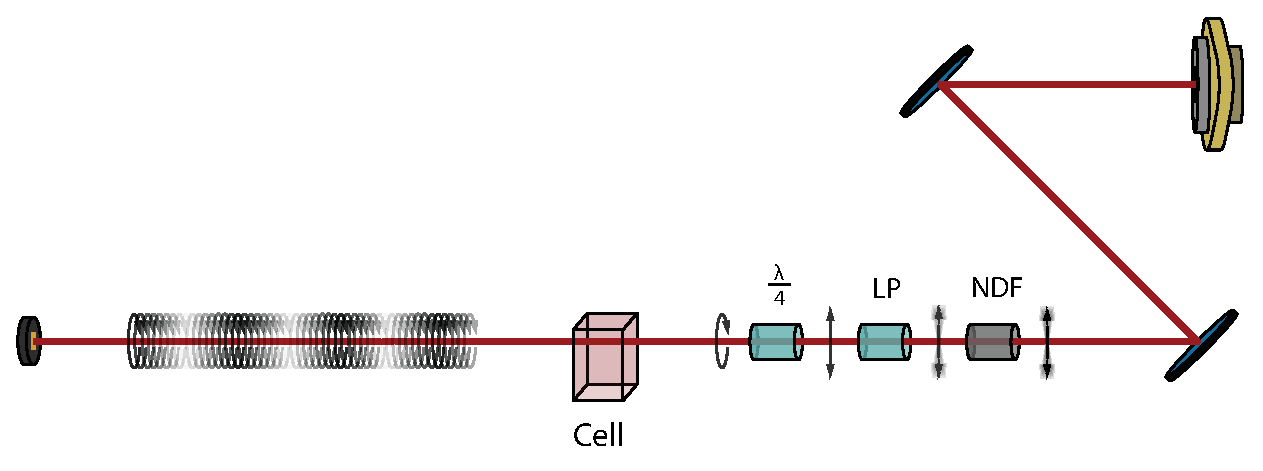
\includegraphics[width=0.9\tw]{figures/magnetometer/SingleBeam.eps}
\caption{The optical path of a single-beam magnetometer.}
\label{fig:SingleBeamOpticalPath}
\end{figure}

Alkali vapor-cell magnetometers use the precession of an ensemble of polarized spins to measure magnetic fields, and that polarization is created by exciting an optical transition which is tied to the the atomic spin state. In the case of our device, circularly polarized 795 nm light is used to excite the D1 transition from rubidium's $5^{2}\textrm{S}_{\sfrac{1}{2}}$ state to a $5^{2}\textrm{S}_{\sfrac{1}{2}}$ excited state (the D1 transition). The electronic states are further split by their total angular momentum, $F = I + J$, where $I$ is the nuclear spin and $J$ is the electron spin. As both $5^{2}\textrm{S}_{\sfrac{1}{2}}$ and $5^{2}\textrm{P}_{\sfrac{1}{2}}$ are singlet states, in both cases the spin quantum number can only take values $m_{f} = \pm \sfrac{1}{2}$. As circularly polarized light carries one unit of spin angular momentum, only transitions where $\Delta F = 1$ are allowed, and so spins are only pumped from the $m_{f} = -\sfrac{1}{2}$ ground state into the $m_{f} = \sfrac{1}{2}$ excited state. Since relaxation back to the ground state is not biased by spin state, relaxing spins are approximately equally likely to transition to either ground state; because spins already aligned along the pump beam ($m_{F} = \sfrac{1}{2}$) are unaffected by pumping, this eventually leads to a buildup of polarization in the $m_{F} = \sfrac{1}{2}$ state dependent upon the relaxation time of the system and the rate of optical pumping.\citep{Seltzer2008,Franzen1957} %Chapter 2.3

An diagram of an optical pumping system is detailed in Fig. \ref{fig:SingleBeamOpticalPath}. The optical pumping rate is adjusted by changing the beam intensity - in this case a neutral density filter is used, but other methods such as crossed linear polarizers can be used for a finer adjustment. A linear polarizer is used to clean up the polarization of the beam, and then the light is passed through a quarter-waveplate with its fast-axis aligned 45$^\circ$ off the axis of linear polarization to produce a circularly polarized beam, which is used to pump the cell. If the polarized spins are in a magnetic field, their state will begin precessing according to $\cos{\omega{}t}\left|+\tfrac{1}{2}\right\rangle + \sin{\omega{}t}\left|-\tfrac{1}{2}\right\rangle$. Since the rate of absorption of the photons is a function of the fraction of the ensemble that is in the $\left|-\tfrac{1}{2}\right\rangle$ state, the laser intensity after the cell will be a function of the pumping rate (constant), the spin absorption cross-section (constant) and the precession frequency (a linear function of magnetic field); by measuring the absorption of the pump beam, it is thus possible to operate a magnetometer in a single-beam configuration. While two-beam configurations are often more sensitive, this is the simplest and likely least expensive option.\cite{shah-natphotonics-2007,Schwindt2007}

\section{Pump-Probe Configuration}
\label{mag.design.pump-probe}
A common way to read out the spin precession rate (and thus the magnetic field) experienced by the alkali metal atoms is to make a measurement of the Faraday rotation of off-resonant, linearly polarized light passed through the cell. When the atomic spins are polarized, alkali metal vapor is a birefringent material, with different indexes of refraction $n_{R}$ and $n_{L}$ for the left and right polarized states of light $\left|R\right\rangle$ and $\left|L\right\rangle$. These indices of refraction are proportional to the population of the spin ground states $\rho\left(+\frac{1}{2}_{y}\right)$ and $\rho(-\frac{1}{2}_{y})$ in the frame of reference aligned along the direction of propagation of the probe beam ($y$). For the effect of the D1 transition, these indices are described by Eqn. \ref{eqn:RefractionIndexSpin}\cite{Seltzer2008}

\begin{equation}
\label{eqn:RefractionIndexSpin}
n_{\pm} = 1 + 2\rho\left(\mp\frac{1}{2}_{y}\right)\left(\frac{nr_{e}c^2f_{D1}}{4\nu}\right)Im\left[V(\nu - \nu_{D1})\right]
\end{equation}

The rotation of linearly polarized light will occur because linearly polarized light aligned along a given direction can be decomposed into an equal superposition of left and right circularly polarized light, with the angle of polarization given by a phase difference between the two:

\begin{equation}
\label{eqn:LinearCircularBasisTransform}
\left|\Theta\right\rangle = \frac{1}{\sqrt{2}}\left[e^{-i\Theta}\left|\circlearrowright\right\rangle + e^{i\Theta}\left|\circlearrowleft\right\rangle\right]
\end{equation}

Thus for a non-zero population difference $\rho\left(+\frac{1}{2}_{y}\right) \neq \rho\left(-\frac{1}{2}_{y}\right)$, the differential retardation of each component introduces some additional phase between the two circularly polarized components, tipping the polarization of the probe beam by an angle $\theta$, given by Eqn \ref{eqn:FaradayRotationAngle}\footnote{One thing to note is that this takes into account only the effect of the D1 transitions. For a more in-depth analysis of the effect which takes into account the D2 transition (relevant in potassium magnetometers), see \textit{Seltzer, 2008, pp 32-37}\cite{Seltzer2008}.}:

\begin{equation}
\label{eqn:FaradayRotationAngle}
\theta = \frac{\pi}{2}\mathrm{ln}(r_ec)\left[\rho\left(+\frac{1}{2}_{y}\right)-\rho\left(-\frac{1}{2}_y\right)\right]\left(-f_{D1}Im[V(\nu-\nu_{D1})]\right)
\end{equation}

For a pump beam along an orthogonal direction ($x$), in the presence of no precession, there is no difference in polarization between the ground states along $y$, as the spin states polarized along $x$ can be decomposed into an equal linear superposition of spins polarized along $y$. An average rotation about the $z$ axis of the ensemble by angle $\tilde{\theta} = \gamma_{S}B_{z}R_{P}$ induced by a magnetic field tips the spins towards the $y$ axis, with populations given by Eqn \ref{eqn:SpinTipPopulations}:

\begin{equation}
\label{eqn:SpinTipPopulations}
|\tilde{\theta}\rangle = \left(cos\tilde{\theta} + sin\tilde{\theta}\right)\left|+\frac{1}{2}_{y}\right\rangle + \left(cos\tilde{\theta} - sin\tilde{\theta}\right)|-\frac{1}{2}_{y}\rangle
\end{equation}

Thus the population difference $P_y = \rho(+\frac{1}{2}_{y}) - \rho(-\frac{1}{2}_{y})$ is:
\begin{align}
\label{eqn:PopulationDifferenceSpinsTipped}
P_y & = & (\cos\tilde{\theta} + \sin\tilde{\theta}) - (\cos\tilde{\theta} - \sin\tilde{\theta}) \\
& = & 2\sin\tilde{\theta}
\end{align}

And for small angles, $2 \sin\tilde{\theta} \approx 2\tilde{\theta}$. Finally, taking this result and inserting it into Eqn \ref{eqn:FaradayRotationAngle}, the Faraday rotation angle for a given average tip angle is:

\begin{align}
\label{eqn:RotationFromTip}
\theta & = & \frac{\pi}{2}\ln{r_ec}(2\sin\tilde{\theta})\left(-f_{D1}Im[V(\nu-\nu_{D1})]\right) \\
& \approx & \frac{\pi}{2}\ln{r_ec}(2\tilde{\theta})\left(-f_{D1}Im[V(\nu-\nu_{D1}]\right)
\end{align}

Which, for small angle and constant frequency is linearly proportional to $\tilde{\theta}$.

\subsection{Balanced Polarimeter}
\label{mag.design.balanced.polarimeter}
\begin{figure}[ht!]
\centering
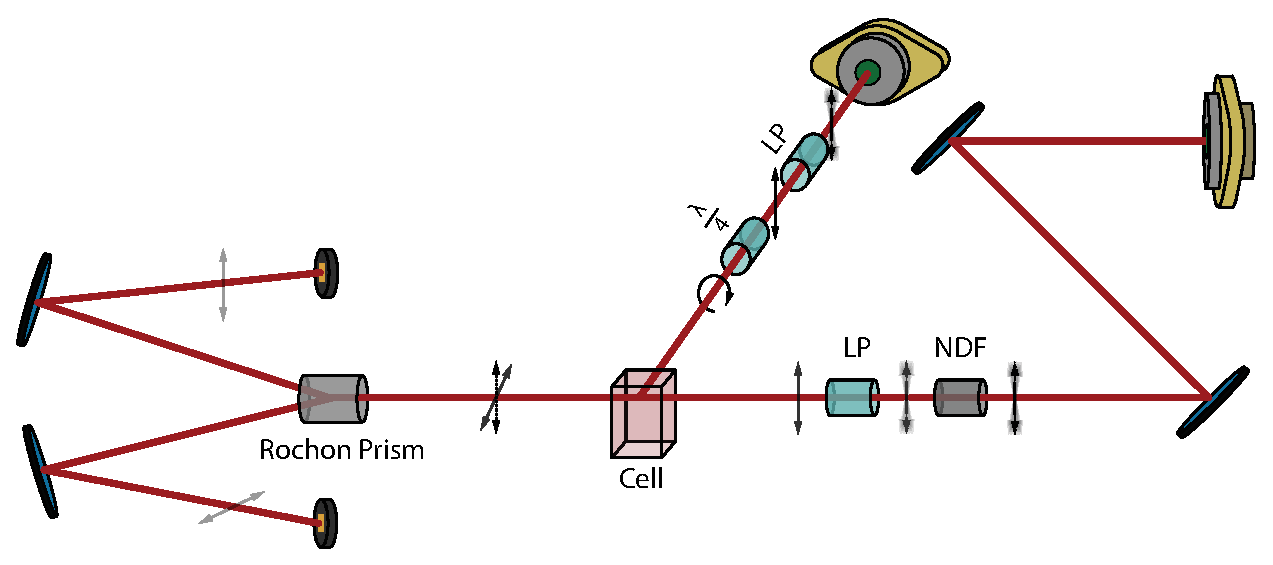
\includegraphics[width=0.9\tw]{figures/magnetometer/BalancedPolarimeter.eps}
\caption{The optical path of a pump-probe magnetometer with a balanced polarimeter used for signal detection.}
\label{fig:BalancedPolarimeterOpticalPath}
\end{figure}
A balanced polarimeter is a simple device for measuring linear polarization, and is the method of choice for our magnetometer due to its high sensitivity. The beam path is shown in \Cref{fig:BalancedPolarimeterOpticalPath}. The beam is first reflected off two dielectric mirrors to provide optimal beam angle and position control, followed by a neutral density filter (or crossed-polarizer), which is used to attenuate the beam to the appropriate value. A linear polarizer with its fast axis aligned with the vertical is used to provide clean, uniform vertical polarization, and then the beam passes through the cell, where the light undergoes a Faraday rotation. Finally, the beam is passed through a Rochon prism whose fast axis is aligned 45\degsym  off vertical, which splits the beam into its diagonal and anti-diagonal components. The beams will have intensities:\citep{Seltzer2008} % Chapter 2.4.2

\begin{eqnarray}
P_D & = & P_{0}\sin^2\left(\frac{\pi}{4} - \theta\right) \\
P_A & = & P_{0}\cos^2\left(\frac{\pi}{4} - \theta\right) 
\end{eqnarray}

Where $\theta$ is the angle of polarization off the vertical axis. By subtracting the current in the diagonal channel from the current in the antidiagonal channel, the result is:

\begin{eqnarray}
P_{D} - P_{A} & = & P_{0}\sin^2(\theta - \frac{\pi}{4}) - P_{0}\cos^2(\theta - \frac{\pi}{4}) \\
& = & \frac{P_{0}\left[]1+\cos\left(2\theta - \frac{\pi}{2}\right)\right]}{2} - \frac{P_{0}\left[1-\cos\left(2\theta - \frac{\pi}{2}\right)\right]}{2} \\
& = & P_{0}\sin\left(2\theta\right)
\end{eqnarray}

And if $2\theta$ satisfies the small angle approximation then $\sin(2\theta) \approx 2\theta$. This gives us a signal given by:

\begin{equation}
P_{D} - P_{A} \approx 2P_{0}\theta
\end{equation}

Since this applies only for small angle $\theta$, it is necessary for the initial input polarization to be ``balanced'', which is to say the pre-rotation beam should be exactly 45\degsym  off the fast axis of the Rochon prism. Because rotating a Rochon prism rotates both output beams, it is often most convenient to simply rotate the linear polarizer used to clean up the beam, as the rotations are small enough that this is unlikely to cause a significant dip in the output intensity.

\subsubsection{Practical Concerns}
\label{mag.design.balanced.polarimeter.practical}
The operation of the balanced polarimeter is characterized by a great deal of symmetry - because it measures very small angles, what's being measured is relatively small differences in two channels with comparatively high absolute signal - the average light incident on each channel is likely to be roughly an order of magnitude larger than the range of linear response. As a result, great care should be taken to avoid asymmetric noise in the detection section between the two channels. 

One such source of noise is clipping - the likely source of clipping noise is angular noise at the beam source, translated into noise on the beam position later, and as such the magnitude of the clipping noise will grow as the length of the beam path grows. As such, while clipping on an iris at the laser source may be acceptable, clipping later in the beam path can easily become a limiting source of noise. This is particularly problematic if the clipping occurs \textit{after} the beam splitting optics, as this will cause largely independent and asymmetric noise on the absolute intensity of each beam. Ideally, the length of the beam path after the beams have been split will be kept as short as possible, and the two arms of the beam preferably kept at equal length.

Another practical issue with balanced polarimeter operation is the possibility of asymmetric response between the two detection channels, which can occur due to any number of asymmetries in the two beam paths - differences in the load resistor, diode response, bias offset voltage, etc. The likely problem with channel asymmetries is that it can lead to a ``false balance'', wherein zero output signal is achieved at a non-zero angle $\theta_{e}$. To first order, the primary effect of a ``false balance'' is that the polarimeter will be operating in a non-linear region. Additional problems can arise if the beams are being operated near the linearity limit of the photodiodes - since a stronger signal is required in one of the two channels, in order to keep both channels operating in the linear region, the beam will then need to be attenuated further than necessary, reducing signal.

There are two main causes of false balance - difference in the response of the electronics and differences in response from the photodiodes themselves. Starting with the electronics, a very likely culprit for inducing false balance will be an imbalance in the load resistances. For load resistors $R_{L1}$ and $R_{L2}$ and deviation $\epsilon_{R}$ defined such that $R_{L1} = R_{L} + \sigma_{R}$ and $R_{L2} = R_{L} - \sigma_{R}$\footnote{This is always the case when $R_{L}$ is the average of $R_{L1}$ and $R_{L2}$ and $\sigma_{R}$ is the ``standard deviation'' of the two values.}, the angle $\theta_{e}$ which makes the channels appear balanced is given by Eqn \ref{eqn:PDResistorLoadIMbalancedAngle}:

\begin{equation}
\label{eqn:PDResistorLoadIMbalancedAngle}
\theta_{e} = \frac{1}{2}\textrm{asin}\left(\frac{\sigma{R}}{R_{L}}\right)
\end{equation}

For the common ``gold band'' type resistor with tolerance $\pm$ 5\%, assuming a typical quadrature addition of errors, a typical $\sfrac{\sigma_{R}}{R_{L}}$ will be $0.05\sqrt{2}$, which gives $\theta_{e} \approx$ \unit[35.4]{mrad}. This particular problem is easy to solve by placing trim-potentiometers in series with the load resistors and actively balancing the resistor channels.

Another potential cause of false balance is differences in the response of each channel's photo-diodes. While the inherent response curves of each photodiode is not necessarily something that anything can be done about, adding in symmetry between the channels and making sure the signal from each channel is individually maximized can go some way towards alleviating this problem. Depending on the photodiodes, there may be some responsivity gradient across the sensitive area, and that will certainly be true if any clipping is occurring. 

In our setup, the response of our DET110 photodiodes seem somewhat sensitive to beam width and position, and so to start we try to keep beam path lengths as close to identical as possible to account for deviations from well-collimated beams (often when using smaller photodiodes, it may also be advantageous to put a lens on the input of the beam-splitting optics to focus near to the photodiode - in this case, beam path length may be a critical factor). The beams are positioned using the output signal of each individual channel - the beam is roughly centered by eye on the photodiode, and then the optimal position is found by iteratively maximizing the signal from each channel with respect to horizontal and vertical position. In this instrument, the angle of incidence is set such that the beams are roughly normal to the sensitive surface (this is estimated by eye, but it's not impossible to use some sort of signal-maximizing feedback to find this angle more precisely).

\subsubsection{Balancing Procedure}
\label{mag.design.polarimeter.balancing}
With issues of false balance hopefully largely accounted for, finding the right balance is largely a matter of adjusting the input polarization of the light. It's best to do this while changing the minimum number of other factors which could affect the polarization, such as the length of the beam path or temperatures or positions of the optics. If the pump beam is operating, the polarization of the light will be sensitive to the magnetic field at the cell, and so the polarimeter is always balanced with the pump beam blocked.

The polarimeter can, in theory, be balanced either by adjusting the beam-splitting optics until they are exactly \unit[45]{\degsym} off axis from the input polarization, but in many (if not all) cases this will affect the path of the output beam and not just the polarization of at least one of the two channels, and so all optics after the beamsplitter would need to be adjusted. Usually it is preferable to adjust the linear polarizer which comes before the cell; the downside of this  method is that the output signal amplitude is a function of the beam rotation - because these rotations are often quite small it is not usually a problem, but it is worth keeping an eye on the power of the post-polarizer beam, and if it becomes too attenuated a half-waveplate can be added before the linear polarizer to tip the polarization into the right alignment.\cite{Wu1986}

Another concern is possible birefringence introduced by the cell glass - which is likely under some strain due to the omnipresent thermal gradients. The birefringent properties of the glass will likely change both the angle of linear polarization and the ellipticity of the beam. This can be represented on the Poincar\"{e} sphere as a a rotation of an arbitrary angle ($\theta_{B}$) about an arbitrary axis ($\mathbf{\hat{u}}$). Using a combination of a linear polarizer (or half-waveplate, depending on the severity of the birefringence) and a quarter-waveplate, the input polarization can be set such that the birefringence of the glass will make the light linear and aligned properly.

One thing to note is that in a balanced polarimeter, probe beam ellipticity should have no biasing effect on the signal, as elliptical components can be decomposed as an equal superposition of horizontal and vertical states (and thus subtract out). Beam ellipticity in the beam leaving the cell will thus only affect the overall signal intensity, and this will likely not be a significant problem for small deviations from linear. However, it can have a significant effect when beam \textit{entering} the alkali vapor is elliptical, as these components will tend to pump the spins and slightly change the vector properties of the magnetometer response (including adding a phantom bias ``field'' along the probe direction). As such, when counter-acting beam ellipticity induced by glass birefringence, the magnetometer response is used for feedback, rather than a measure of the beam balance.

There are two main methods for accounting for beam ellipticity. The primary method looks at the magnetometer signal with the pump beam blocked - some fraction of the spins become polarized along the direction of the probe beam ($y$), and thus the magnetometer becomes sensitive to fields along $x$ and $z$. In this method, an oscillating magnetic field is induced\footnote{Usually this field much larger than the test signal - our typical test signal is \unit[62.7]{pT$_{RMS}$} for sensitivity testing and \unit[6.27 or 62.7]{nT$_{RMS}$} for detection of ellipticity} and the quarter waveplate and linear polarizer are iteratively adjusted until the oscillations are no longer detectable and the DC level is balanced.

The other method for accounting for beam ellipticity is to look at the lineshape of the magnetometer response. A slow ($\approx$ \unit[1-3]{Hz}) triangle wave is applied with an amplitude much greater than the magnetometer's region of linear response - this should result in a Lorentzian lineshape in the magnetometer response. This lineshape is affected by many factors - making it a somewhat less specific optimization parameter, but still possibly more sensitive - and an elliptical probe beam will induce asymmetry between the Lorentzian lobes.

\subsection{Photoelastic Modulator-based Polarimeter}
\label{mag.design.pem}

\begin{figure}[ht!]
\centering
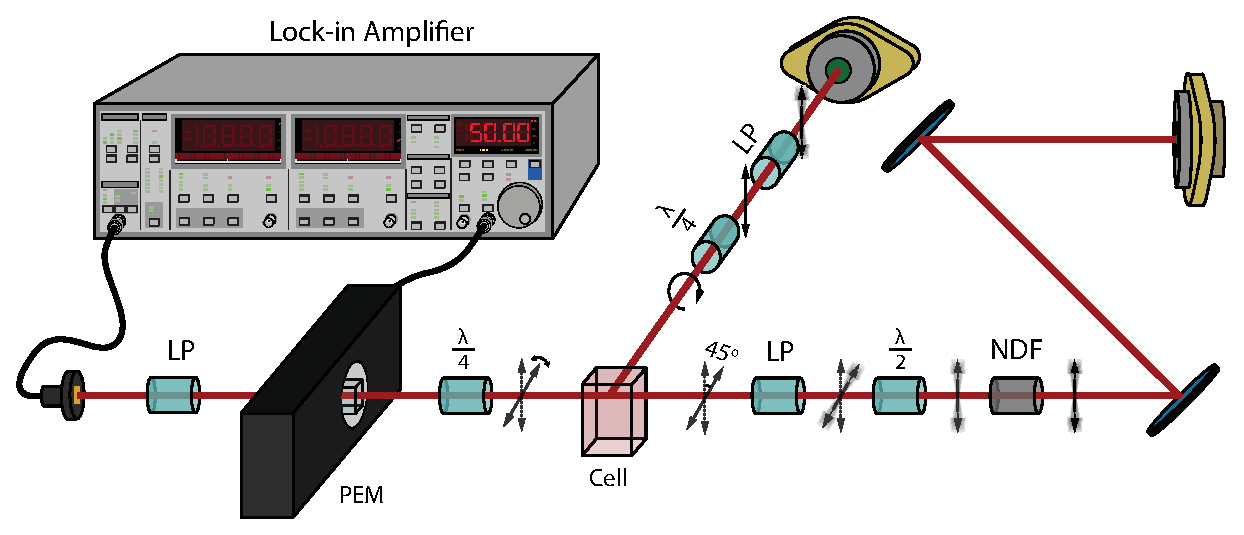
\includegraphics[width=0.9\tw]{figures/magnetometer/PEMSetup.eps}
\caption{The optical path of a pump-probe magnetometer with a PEM-based polarimeter.}
\label{fig:PEMOpticalPath}
\end{figure}

\begin{figure}[ht!]
\centering
\begin{subfigure}[h]{0.3\tw}
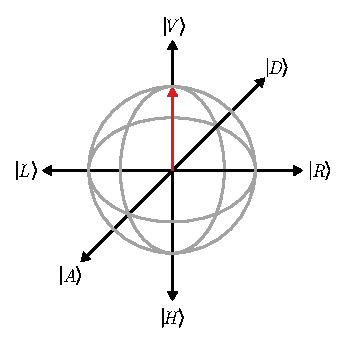
\includegraphics[width=\tw]{figures/magnetometer/PC-Step1.eps}
\caption{}
\label{fig:PEMPCStep1}
\end{subfigure}
\begin{subfigure}[h]{0.3\tw}
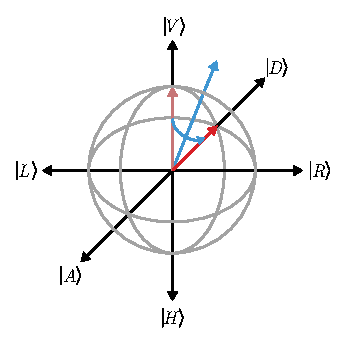
\includegraphics[width=\tw]{figures/magnetometer/PC-Step2.eps}
\caption{}
\label{fig:PEMPCStep2}
\end{subfigure}
\begin{subfigure}[h]{0.3\tw}
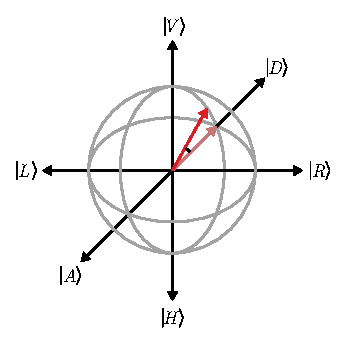
\includegraphics[width=\tw]{figures/magnetometer/PC-Step3.eps}
\caption{}
\label{fig:PEMPCStep3}
\end{subfigure}
\newline
\begin{subfigure}[h]{0.3\tw}
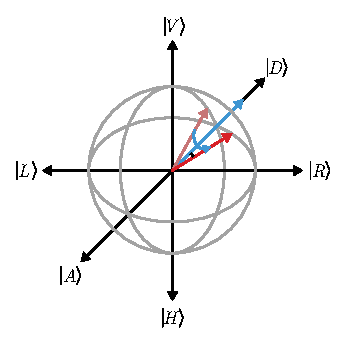
\includegraphics[width=\tw]{figures/magnetometer/PC-Step4.eps}
\caption{}
\label{fig:PEMPCStep4}
\end{subfigure}
\begin{subfigure}[h]{0.3\tw}
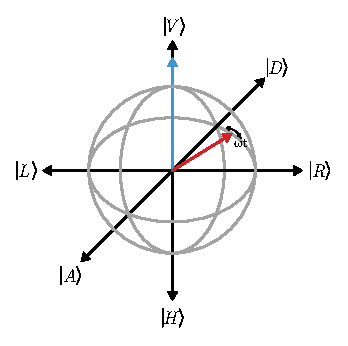
\includegraphics[width=\tw]{figures/magnetometer/PC-Step5.eps}
\caption{}
\label{fig:PEMPCStep5}
\end{subfigure}
\caption{A Poincar\'{e} sphere representation of the polarization of the laser beam throughout the experiment. Light is initially linearly polarized vertical (\ref{fig:PEMPCStep1}), the half-waveplate tips it 45\degsym to lie along the diagonal (\ref{fig:PEMPCStep2}). Passing through the cell causes the light to tip linearly some small angle (\ref{fig:PEMPCStep3}). Passing the light through a quarter-waveplate with fast axis aligned with the diagonal, the light is tipped into the $|D\rangle$-$|R\rangle$ plane (\ref{fig:PEMPCStep4}). Finally the PEM modulates the ellipticity of the beam at frequency $\omega$ (\ref{fig:PEMPCStep5}), and for small Faraday rotations $\theta$, the amplitude second harmonic of the projection onto the anti-diagonal should be linearly proportional to $\theta$.}
\label{fig:PEMPC}
\end{figure}
Another method for measuring the probe beam polarization uses a photo-elastic modulator (PEM)-based polarimeter, wherein the input light's ellipticity is modulated by the PEM and the linear component at the characteristic frequency is measured (\Cref{fig:PEMOpticalPath}). As the measurement is made at higher frequency, this has the potential advantage of avoiding some forms of low-frequency noise that may be present in other methods of polarimetry.

A Poincar\'{e} sphere representation of the beam polarization during the experiment is shown in \Cref{fig:PEMPC}. The probe beam light passes through two mirrors to give maximum control over the positioning of the light, and as before, passes through a neutral density filter (NDF), which is used to set the optimal beam attenuation. Next a half-waveplate with its fast axis set at \unit[22.5]{\degsym}  off vertical is used to rotate the light to \unit[45]{\degsym} off vertical, and the beam is then cleaned up with a linear polarizer set \unit[45]{\degsym}  off vertical (\Cref{fig:PEMPCStep2}). Note that because this polarizer is present, if the half-waveplate is not present, the only consequence is that the beam will be further attenuated by a factor of approximately 2. 

Next, the \unit[45]{\degsym} linearly polarized light passes through the cell and undergoes a small-angle Faraday rotation (\Cref{fig:PEMPCStep3}), after which it is passed through a quarter-waveplate with its fast axis aligned \unit[45]{\degsym} off vertical (aligned with un-rotated light) --- this tips the polarization into the $|D\rangle$-$|R\rangle$ plane (\Cref{fig:PEMPCStep4}), thus translating linear rotation into ellipticity. After this, the light passes through the PEM, which modulates the ellipticity of the beam at the characteristic reference frequency (\Cref{fig:PEMPCStep5}). Finally, the beam passes through a linear polarizer aligned \unit[45]{\degsym} off vertical, selecting a projection of the light onto the $|D\rangle$ axis, which is then fed into a photodiode signal, the intensity of which is given by

\begin{equation}
\sin^{2}\left(\delta\theta + \beta\sin(\omega{}t)\right),
\label{eqn:PEMSignalEquation}
\end{equation}

where $\delta\theta$ is the angle of the Faraday rotation and $\beta$ and $\omega$ are the amplitude and frequency of the PEM modulation, respectively. The signal is fed into a lock-in amplifier synchronized with the PEM, and so the output of the lock-in amplifier, for small angles, is linearly proportional to $\delta\theta$, and insensitive to noise not resonant with the frequency $\omega$ (in our case, the frequency used was $\approx$\unit[50]{kHz}).

% \section{Beam Optimization}
% \label{mag.design.beam.optim}
% The pump and probe beams each have an optimal combination of power and frequency which provide the best magnetometer signal, and it is usually best to discover the instrument settings which most closely approximate these optima by iteratively optimizing the magnetometer signal. The power and frequency for both beams are determined by the laser diode temperature and current controller\footnote{In our instrument, a Thorlabs ITC 502 Laser Diode Temperature and Current controller was used.}, with power determined by the driver current and the resonance frequency tuned by modulating the diode temperature. The polarization is modulated by the optics used in the particular beam configuration. 

%\section{Magnetic Shielding}
%\label{mag.design.shields}
%In most human-created environments, local magnetic field noise and variation due to the omnipresence of magnetic materials and electrical devices are often significantly higher than the fundamental sensitivity of the magnetometer. Where fundamental magnetometer sensitivity is on the order of \unitfrac[0.1]{fT}{\rHz} (\unitfrac[1]{pG}{\rHz}), low-frequency noise (1 Hz) in the Earth's field can be on the order of \unitfrac[2]{pT}{\rHz} (\unitfrac[10]{nG}{\rHz}).\needcite{Citation for the low frequency noise from the Earth's field. New book from Dima}\cite{Nichols1988} Among the most common strategies for eliminating this noise is the use of high permeability magnetic shielding, particularly $\mu-$metal - a generic name for a class of extremely high permeability nickel-iron alloys.
%
%High permeability metal shields can attenuate DC magnetic fields by concentrating magnetic flux within the conduction path of the shields.  

%

\end{document}